\section*{Introduction}

This document contains the definition of the hardware configuration of the COACHES robots and the communication infrastructure. In particular, the hardware set-up of the robot is described in Section 1, the communication infrastructure in Section 2, while Section 3 illustrates the robot design.

The robots are under development by Algorithmica company\footnote{www.algorithmica.it} and they are expected to be delivered in Fall 2015.


\section{Robot Hardware Set-up}

The design of the COACHES robots has been carried out considering the requirements of the project, the environment in which they will operate, and the definition of the use cases.
Moreover, the proposed solution is based on the experience gained in building and using DIAGO robot\footnote{https://sites.google.com/a/dis.uniroma1.it/diago} at Sapienza University.

In this section, we report the main hardware components of the robot and their connections.


\subsection{Robot Hardware}

Each robot will be assembled by using the following main components.
The design of the robot is described in a later section in this document.


\subsubsection{Robot base}
The main robotic platform consists of a Segway's RMP210, shown in Fig. \ref{fig:segway}.
It is a non-balancing platform with two propulsion wheels which can operate stably in indoor environments via a third caster wheel. The base is able to load up to 45 kg, suitable to carry out the transportation tasks of the use cases defined in deliverable D5.2. Below, we describe the main technical characteristics of the platform:
\begin{itemize}
\item Dimensions: 625 mm x 637 mm x 481 mm
\item Weight: 52 kg
\item Max payload: 45 kg
\item Max speed: 8 m/s
\item Battery capacity: 380 Wh
\item Battery charge time: 2-3 hours
\item Run time: Up to 24 hours
\end{itemize}

\begin{figure}[h!]
\begin{center}
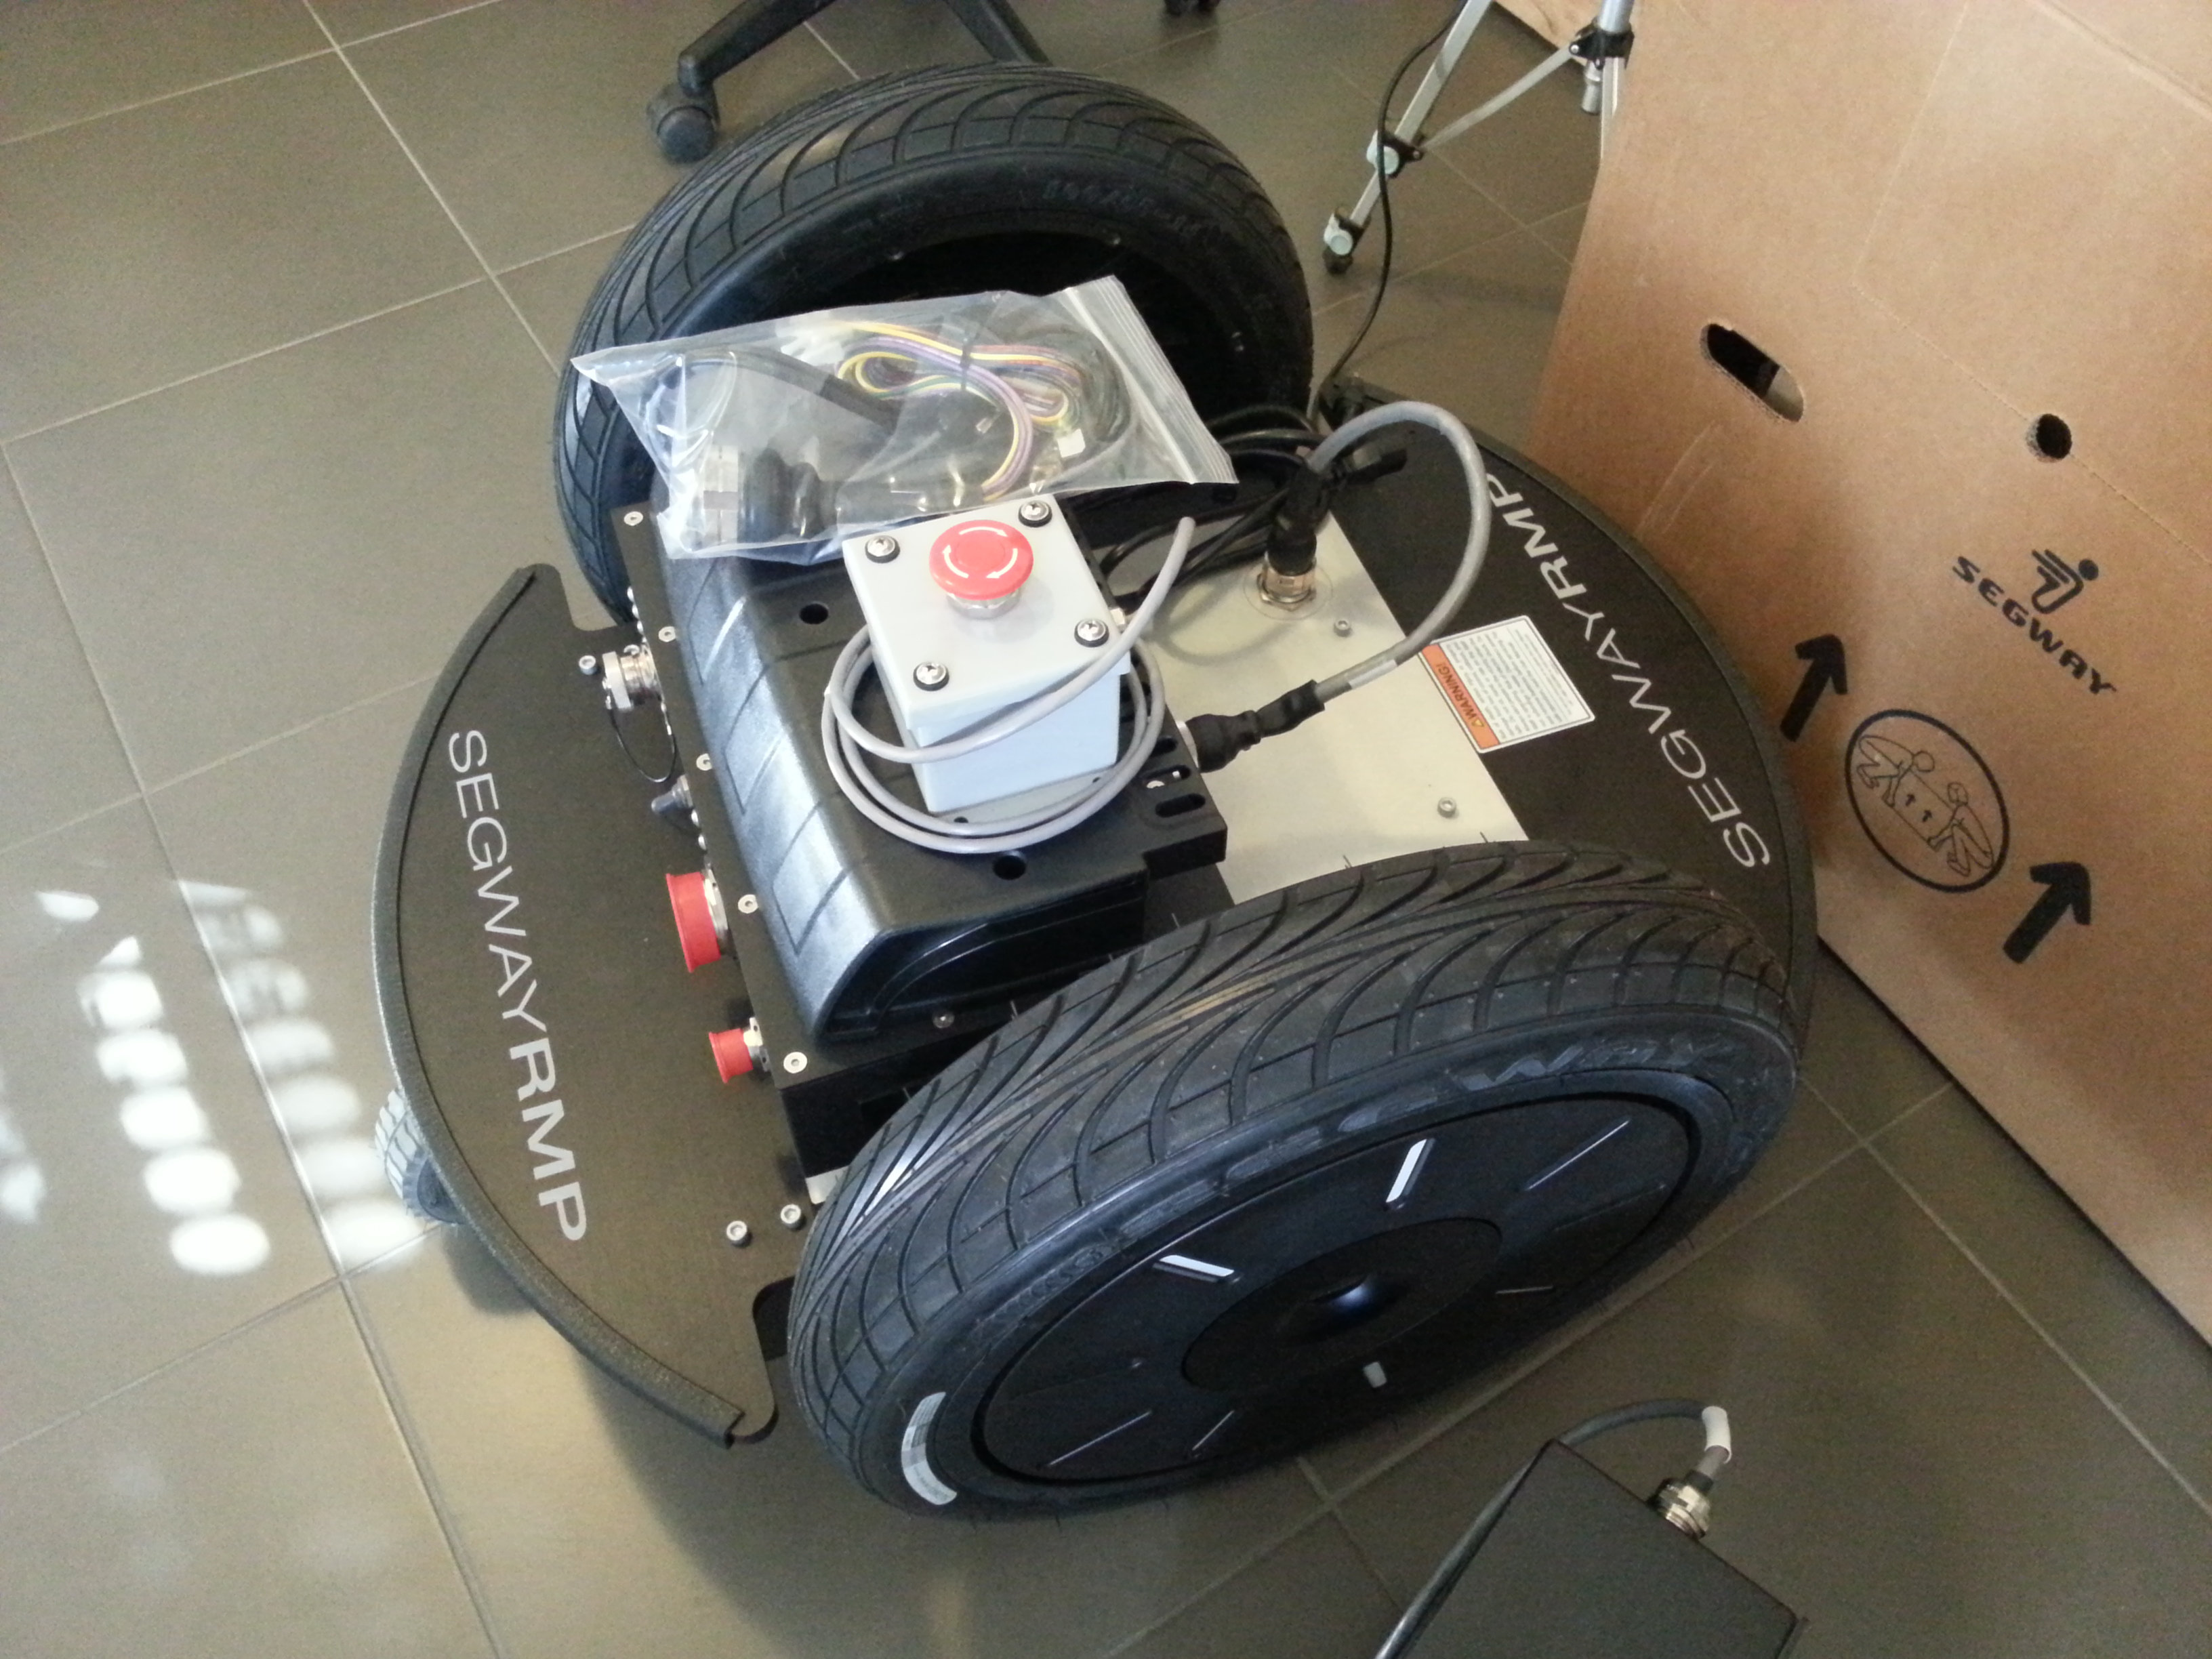
\includegraphics[height=5cm]{fig/segway_rmp210.jpg}
\end{center}
\caption{Segway RMP210 mobile platform.}
\label{fig:segway}
\end{figure}

\subsubsection{On-board sensors}

{\bf Laser range finders}
Two laser range finders equipped on the front (Hokuyo UTM-30-LX) and back (Hokuyo URG-04LX-UG01) sides of the robot will be used for robot localization, obstacle avoidance and potentially people tracking.

\begin{tabular}{|c|c|c|}
\hline
\bf{Model No.}& \bf{UTM-30-LX} & \bf{URG-04LX-UG01}\\
\hline
\bf{Power source} & 12VDC±10\% & 5VDC±5\%(USB Bus power)\\
\hline
\bf{Detection Range} & 0.1 to 30m (Max. 60m) & 20 to 5600mm\\
\hline
\multirow{2}{*}{\bf{Accuracy}}
 & 0.1 to 10m:$\pm$30mm  & 60 to 1,000mm : $\pm$30mm\\
 & 10 to 30m:$\pm$50mm & 1,000 to 4,095mm : $\pm$3\% of measurement\\
\hline
\bf{Scan Angle} & 270$^{\circ}$ & 240$^{\circ}$\\
\hline
\bf{Angular Resolution} & 0.25$^{\circ}$ & 0.36$^{\circ}$\\
\hline
\bf{Scan Time} & 25ms  & 100ms\\
\hline
\bf{Weight} & Approx. 370g  & Approx. 160g \\
\hline
\end{tabular}

{\bf would be interesting to know which is the actual scanning angle due to the cover.}


\begin{figure}[h!]
\begin{center}
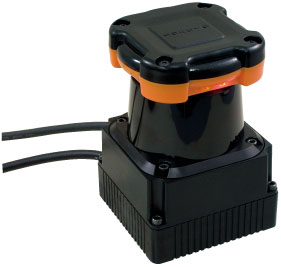
\includegraphics[height=3cm]{fig/utm30lx.jpg}
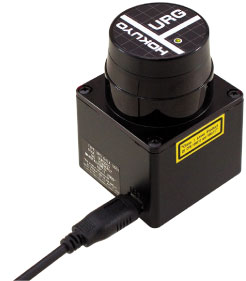
\includegraphics[height=3cm]{fig/urg04lxug01.jpg}
\end{center}
\caption{Hokuyo UTM-30-LX and URG-04LX-UG01 laser range finders.}
\label{fig:segway}
\end{figure}

{\bf Cameras: 2 ASUS Xtion pro Live, Logitech C920}



\subsubsection{Human-Robot Interfaces}

Speakers:

Microphone: Microphone RODE NTG-2  (directional microphone) ...

Tablet: Microsoft Surface Pro 2

\subsubsection{Additional devices}
PC laptop: HP EliteBook 820 G2
SBC: 3 Odroid C1
Network switch for internal communication and external wireless communication




\subsection{Device Connections}

Robot, 2 Laser, 3 Cameras -USB- 2 Bananas

3 Odroid  -Ethernet- Net Switch

Laptop, Tablet -Ethernet- Net Switch

Microphone -USB- Tablet

Speakers -audio jack- Tablet

External devices -Wireless- Net switch



\subsection{Device drivers}

thin\_drivers ...






